\documentclass[12pt, a4paper]{article}
\usepackage[utf8]{inputenc}
\usepackage{a4wide}
\usepackage{color, amssymb}
\usepackage[margin=2.5cm]{geometry}
\usepackage{listings, amsmath, float}
\usepackage{subfig}
\usepackage{textcomp}
\renewcommand{\baselinestretch}{1.5}
\setlength\parindent{24pt}
\usepackage{graphicx, cancel}
\graphicspath{ {./images/} }

\title{First Project}
\author{Odysseas Stavrou, Olga Tsirou}
\date{October 2020} 

\begin{document}
\noindent\rule{\textwidth}{1.5pt}

\begin{center}
    {\bf Telecommunication Systems I} \\ 
    Report of the 3rd Project\\
    Olga Tsirou 2018030061\\
    Odysseas Stavrou 2018030199\\
    December 2020\\
    Technical University of Crete\\
    Prof.:\ A. P. Liavas 
\end{center}
\noindent\rule{\textwidth}{1.5pt}

\begin{enumerate}
    \item[A.] \textbf{\underline{Study of 8-PSK fundamentals}}
    \begin{enumerate}
        \item[1.] \underline{Data Creation:}\\
        MATLAB's \textbf{randi} function was used to produce the binary sequence, 
        consisting of \(3N\) equally probable bits. 
        \begin{figure}[H]
            \centering
            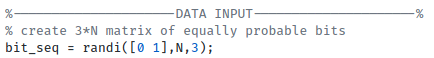
\includegraphics[scale=0.9]{bit_cre.png}
        \end{figure}
        \item[2.] \underline{Encoding:}\\
        The bits were encoded into 8-PSK symbols using the following Gray table
        and the following function. Each one of the 8 possible symbols is described 
        as a column vector as shown below:
            \[\textbf{X}_n = 
            \begin{bmatrix}
                X_{I,n}\\
                X_{Q,n}
            \end{bmatrix}
            =\begin{bmatrix}
                \cos(\frac{2\pi m}{8})\\
                \sin(\frac{2\pi m}{8})
            \end{bmatrix}, \quad m \in [0,7]\]

            \begin{center}
                \begin{tabular}{ | c | c | c | } 
                    \hline
                    Bits & \(X_I\) & \(X_Q\) \\ 
                    \hline
                    000 & \(\cos(\frac{2\pi0}{8})\) & \(\sin(\frac{2\pi0}{8})\) \\ 
                    \hline
                    001 & \(\cos(\frac{2\pi1}{8})\) & \(\sin(\frac{2\pi1}{8})\) \\ 
                    \hline
                    011 & \(\cos(\frac{2\pi2}{8})\) & \(\sin(\frac{2\pi2}{8})\) \\ 
                    \hline
                    010 & \(\cos(\frac{2\pi3}{8})\) & \(\sin(\frac{2\pi3}{8})\) \\ 
                    \hline
                    110 & \(\cos(\frac{2\pi4}{8})\) & \(\sin(\frac{2\pi4}{8})\) \\ 
                    \hline
                    111 & \(\cos(\frac{2\pi5}{8})\) & \(\sin(\frac{2\pi5}{8})\) \\ 
                    \hline
                    101 & \(\cos(\frac{2\pi6}{8})\) & \(\sin(\frac{2\pi6}{8})\) \\ 
                    \hline
                    100 & \(\cos(\frac{2\pi7}{8})\) & \(\sin(\frac{2\pi7}{8})\) \\ 
                    \hline
                \end{tabular}
            \end{center}  
            \begin{figure}[H]
                \centering
                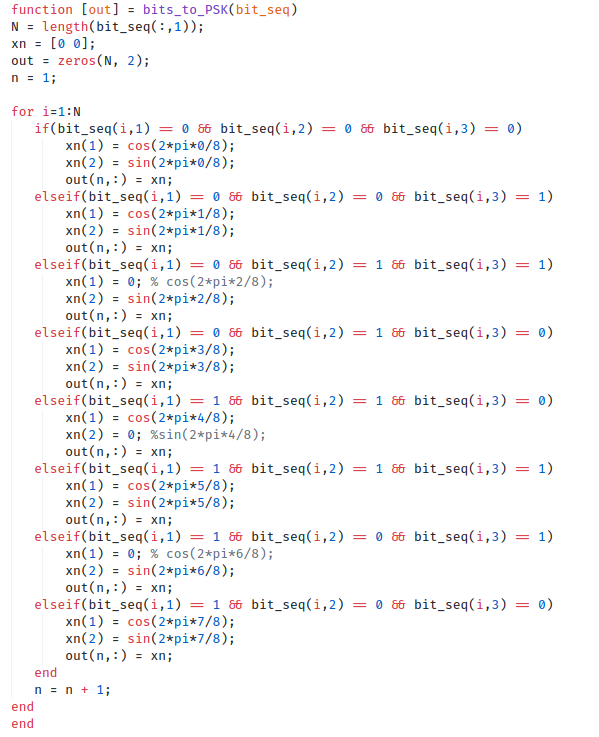
\includegraphics[scale=1]{bit2psk.png}
            \end{figure}
            Note that since MATLAB approximates \(\pi \), some functions like \(\cos(\frac{2\pi2}{8})\) had to be hard-coded to 0.
        \item[3.] \underline{Modulation:}\\
        Convolving the symbols into the \(\phi(t)\) function, produces the following 
        graph and periodogram.
        \begin{figure}[H]
            \centering
            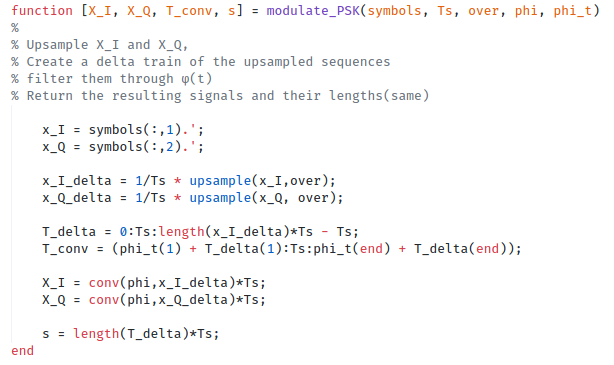
\includegraphics[scale=0.8]{mod_fil.png}
        \end{figure}
        \begin{figure}[H]
            \centering
            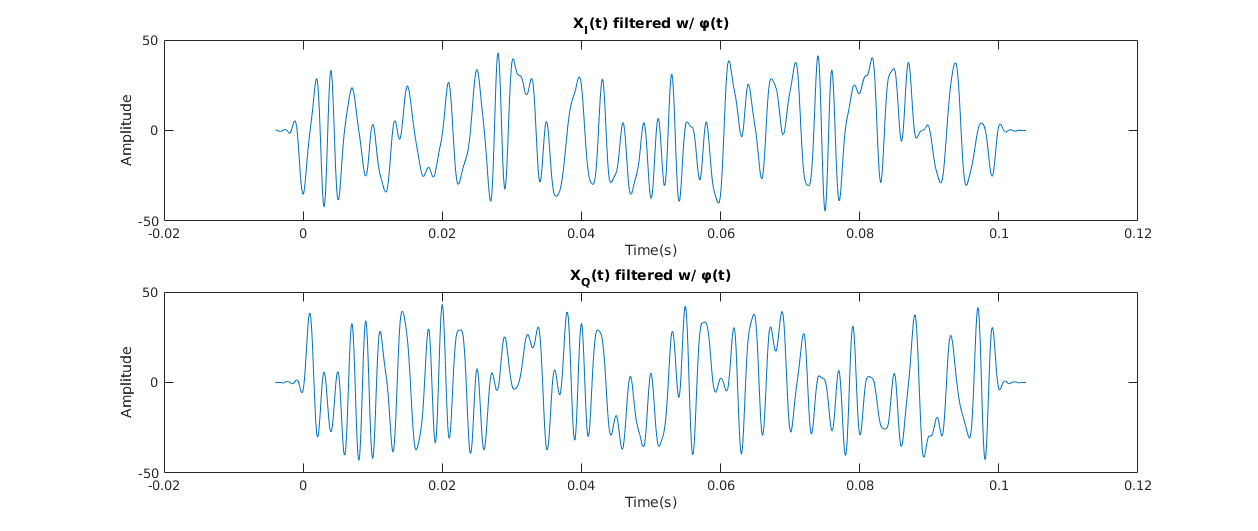
\includegraphics[width=\textwidth]{filter_first.png}
            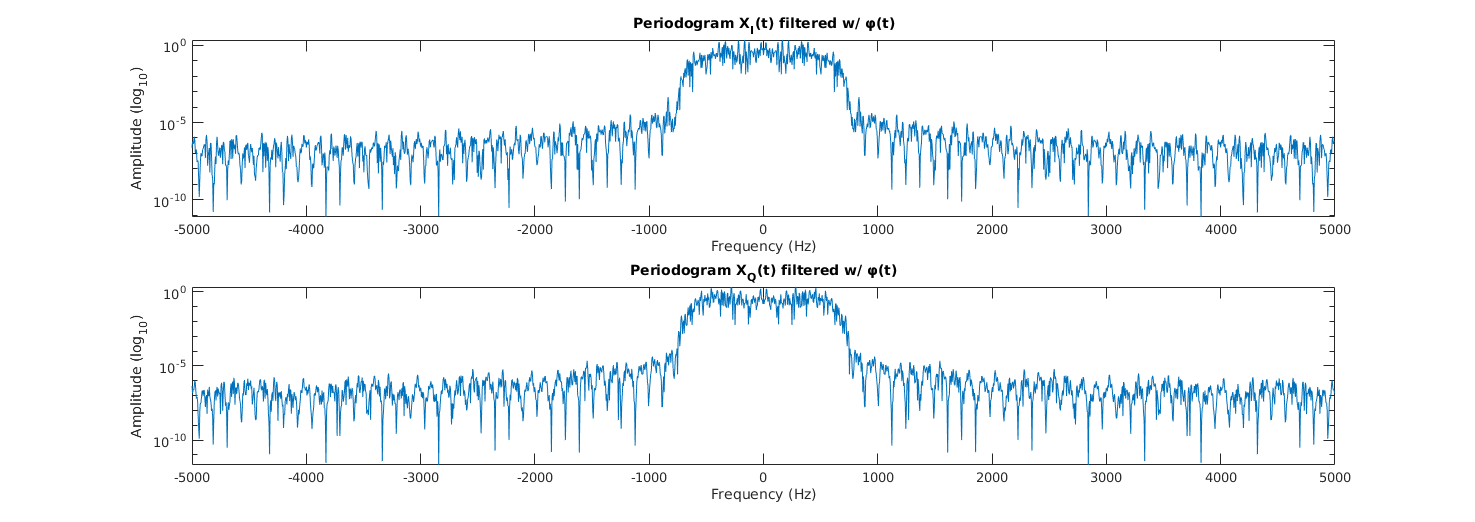
\includegraphics[width=\textwidth]{perio_filter.png}
        \end{figure}
        \item[4.] \underline{Carrier Wave:}\\
        In order to transmit the signal at a certain frequency \(f_0\), 
        it needs to be multiplied with a sine-wave of frequency \(f_0\). Since the information is coded into
        the phase of the signal, it can be observed that each time there is a phase shift, the transmission 
        symbol has changed.
        \begin{figure}[H]
            \centering
            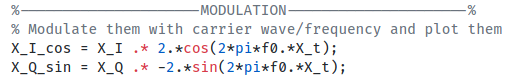
\includegraphics[scale=0.9]{cos_mult.png}
        \end{figure}
        \begin{figure}[H]
            \centering
            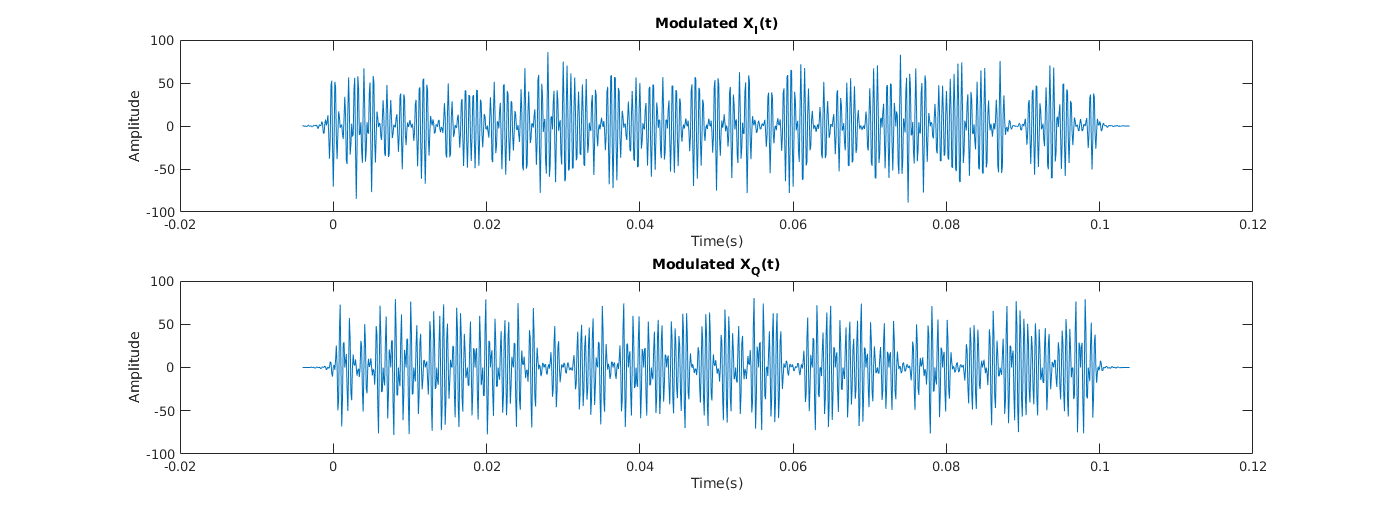
\includegraphics[width=\textwidth]{modu.png}
            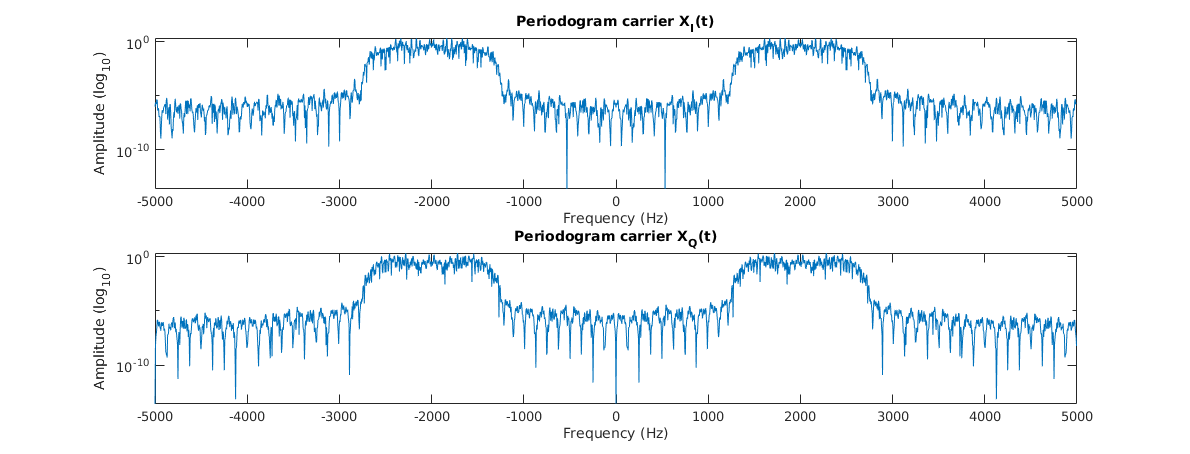
\includegraphics[width=\textwidth]{periodo_modu.png}
        \end{figure}
        \item[5.] \underline{Channel Input:}\\
        Adding the two signals together results in the final transmission signal \(X(t)\). A slight amplification
        can be observed due to summing the above signals. Plotting the periodogram of \(X(t)\) proves that the frequency is 
        the same as the carrier's (\(f_0 = 2KHz)\)
        \begin{figure}[H]
            \centering
            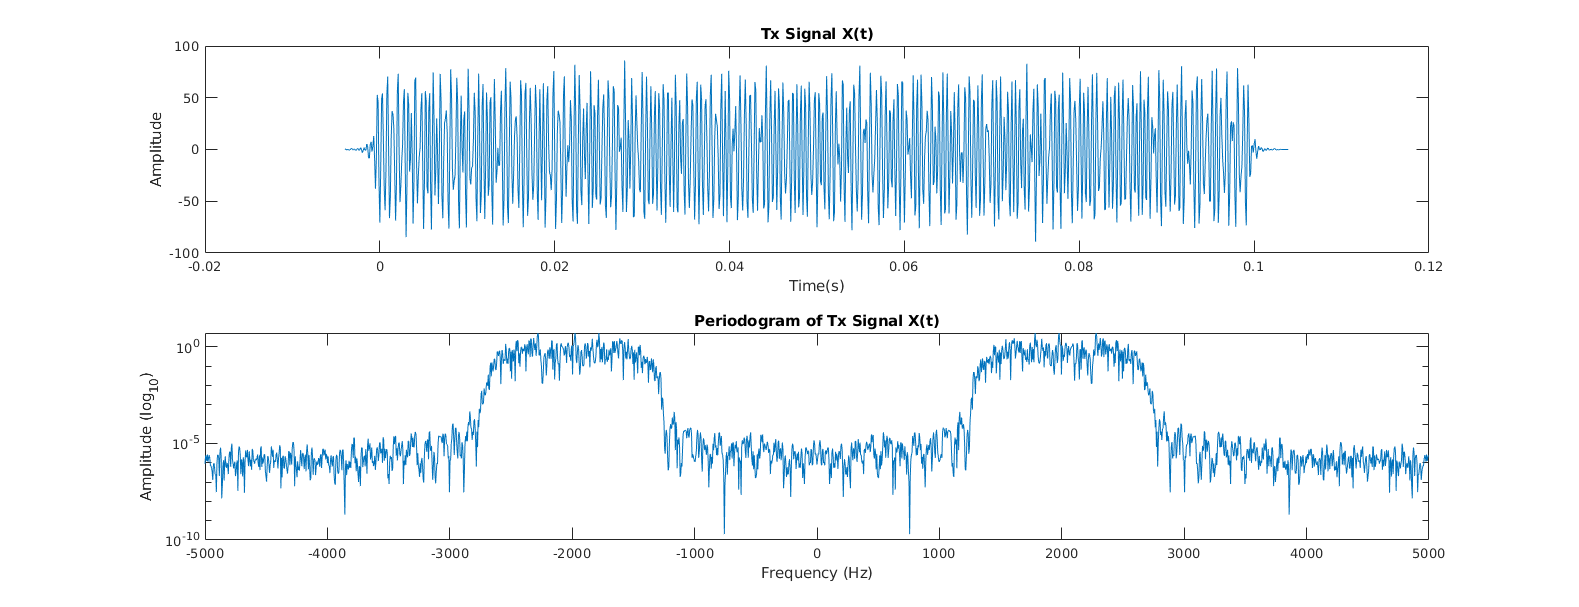
\includegraphics[width=\textwidth]{tx.png}
        \end{figure}
        \item[6.] Assuming an ideal channel, no amplification/attenuation is expected and also perfect synchronization is achieved.
        \item[7.] On the receiver's side the signal \(Y(t)\) arrives with some random noise embedded to it. In this case with a signal
        to noise ratio of 20dB.
        \begin{figure}[H]
            \centering
            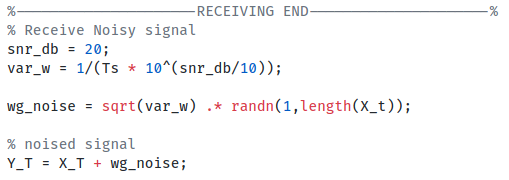
\includegraphics[scale=0.9]{noisy.png}
        \end{figure}
        \begin{figure}[H]
            \centering
            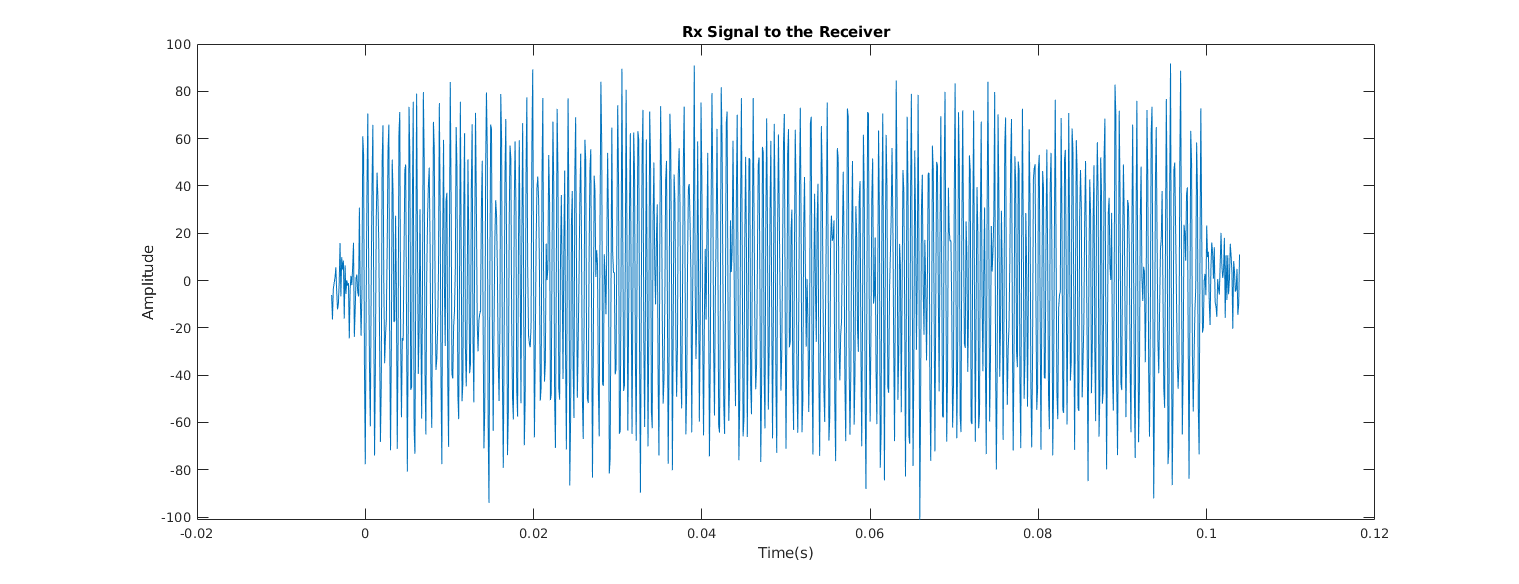
\includegraphics[width=\textwidth]{rx.png}
        \end{figure}
        \item[8.] \underline{Demodulation:}\\
        Multiplying \(Y(t)\) with the same carrier signals used in (4.), splits the signal so that the symbols can be 
        derrived. Studying their plotted periodograms, one could observe that the signal has returned to its baseband form. There 
        are still some lobes around the frequencies of the carrier waves that should be filtered.
        \begin{figure}[H]
            \centering
            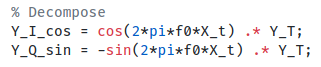
\includegraphics[scale=1]{mult2.png}
        \end{figure}
        \begin{figure}[H]
            \centering
            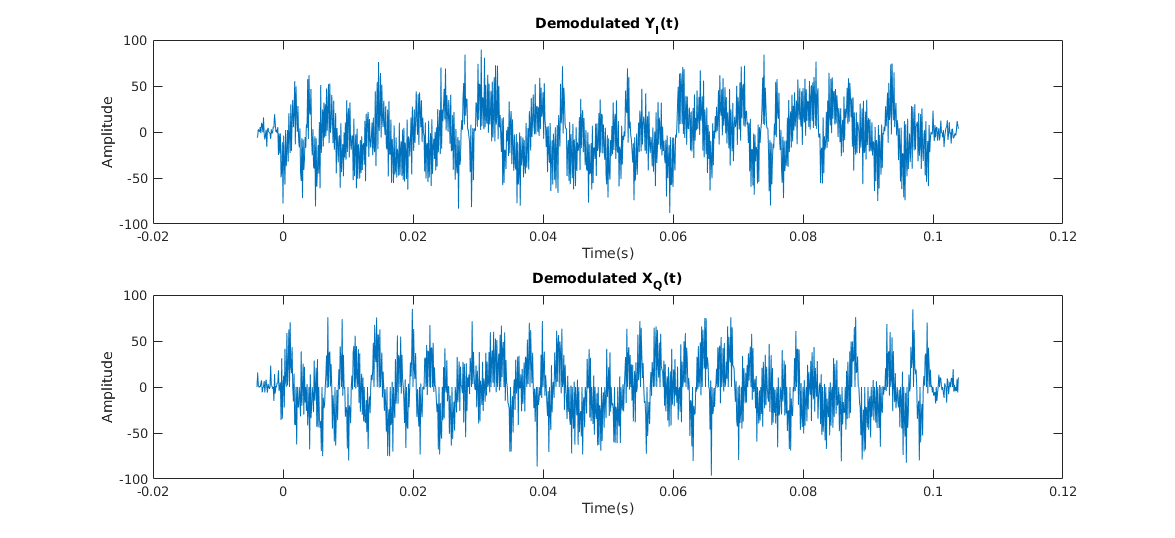
\includegraphics[width=\textwidth]{Y_I_Q_demo.png}
            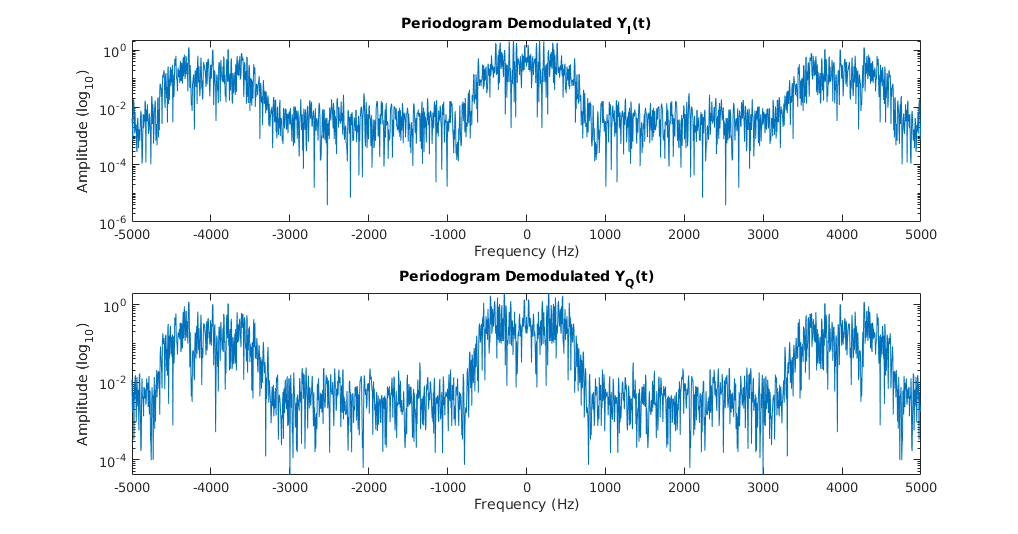
\includegraphics[width=\textwidth]{Y_I_Q_periodogram_demo.png}
        \end{figure}
        \item[9.] \underline{Filtering:}\\
        By filtering the two signals that were demodulated in the previous step, almost identical (due to noise) symbols (with (3.)) are derrived.
        \begin{figure}[H]
            \centering
            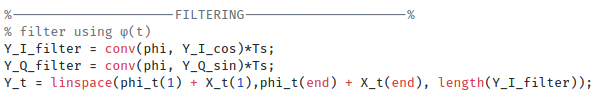
\includegraphics[scale=0.75]{conv_fil.png}
        \end{figure}
        \begin{figure}[H]
            \centering
            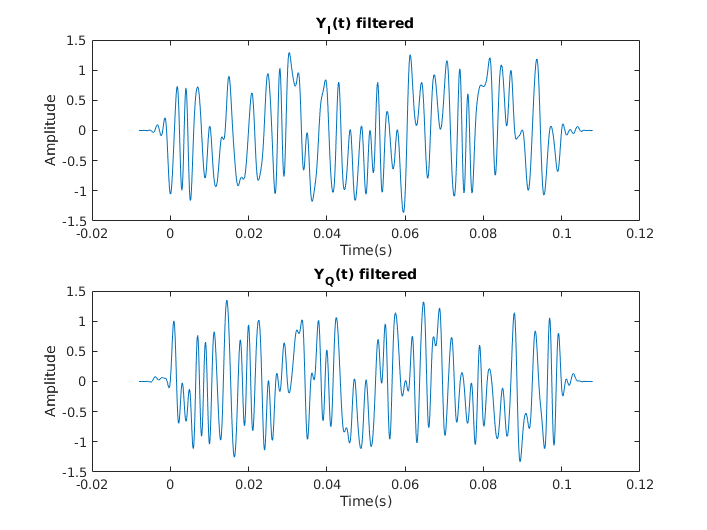
\includegraphics[scale=0.75]{Y_I_Q_filtered_after.png}
        \end{figure}
        \begin{figure}[H]
            \centering
            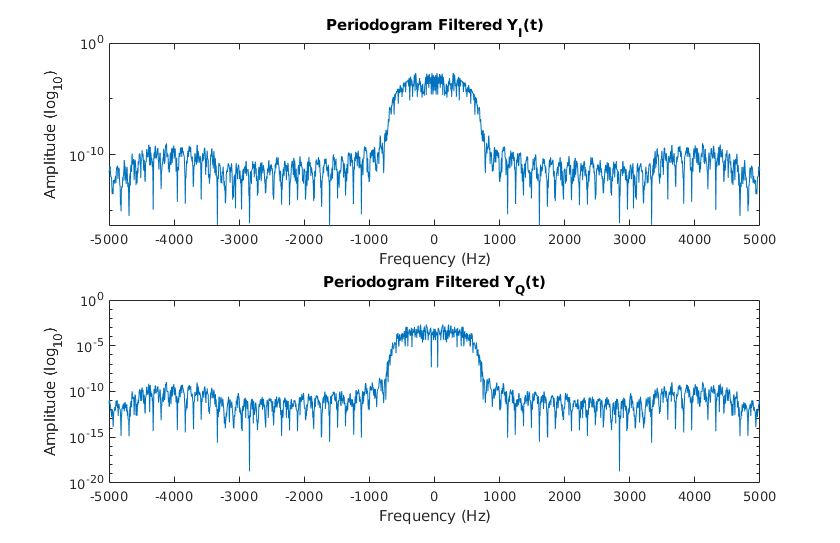
\includegraphics[scale=0.7]{periodo_filter_after.png}
        \end{figure}
        Indeed, after filtering the lobes disappeared.
        \item[10.] \underline{Downsampling:}\\
        Using MATLAB's \textbf{downsample} and \textbf{scatterplot} functions the zeros added by \textbf{upsample} are removed and then the symbols 
        are graphed on the unit-circle. 
        Depending on the SNR (signal to noise ratio) the derrived symbols are closer to, or more randomly scattered around their respective regions.\\
        Note the tail cutting of the convolutions to achieve the correct time vector.
        \begin{figure}[H]
            \centering
            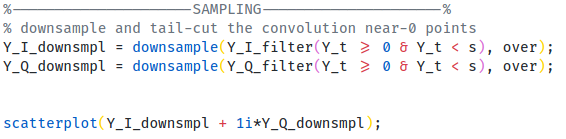
\includegraphics[scale=0.9]{down.png}
        \end{figure}
        \begin{figure}[H]
            \centering
            \subfloat[\centering Received Symbols]{{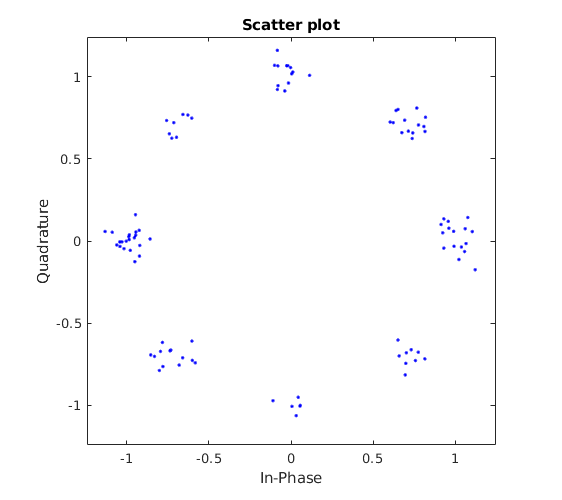
\includegraphics[width=7.5cm]{scatter_after.png} }}%
            \quad
            \subfloat[\centering Original Symbols]{{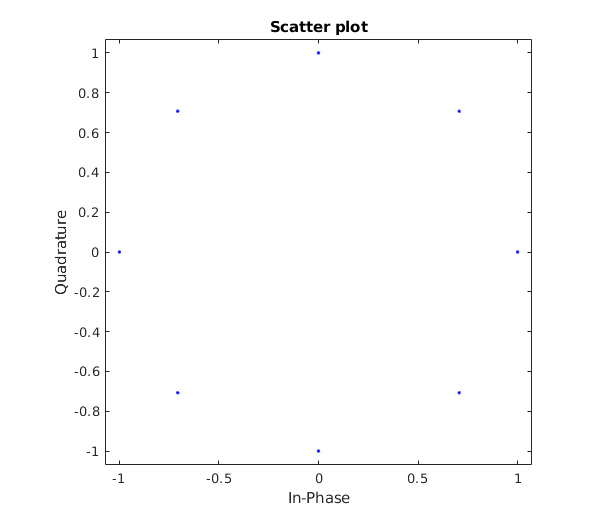
\includegraphics[width=7.5cm]{scatter_orig.png} }}%
            \label{fig:example}%
        \end{figure}
        \item[11.] \underline{Detecting and Decoding Symbols:}\\
        The following function takes each derrived symbol and by using the ``Closest Neighbour Rule'' determines the symbol's actual values.
        To correctly decide the symbol, boundaries are ``drawn'' on the unit circle depicting their regions. If a symbol falls anywhere in 
        that region, then it automatically gets reassigned the correct symbol values.\\
        For each of the 8 possible symbols as a centre, a boundary is a straight line from the circle's center that creates a \(\pm 22.5^\circ \) angle
        from the symbol.
        \begin{figure}[H]
            \centering
            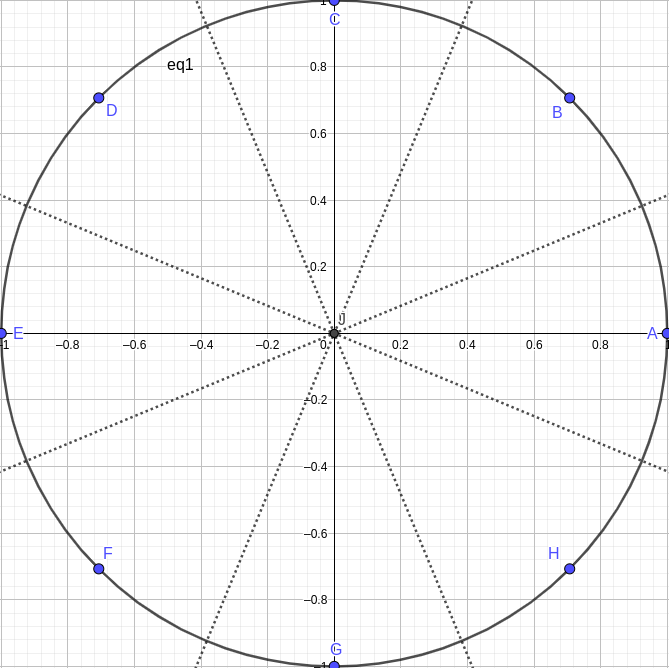
\includegraphics[scale=0.5]{geogebra.png}
        \end{figure}
        The dottet lines represent the boundary limits of each Symbol in its respective region.
        MATLAB's \textbf{atan2, wrapTo2Pi, rad2deg} functions were used in order to determine the angle in [0, \(360^{\circ}\)).\\
        After that all symbols are decoded using the table in (2.). 
        \begin{figure}[H]
            \centering
            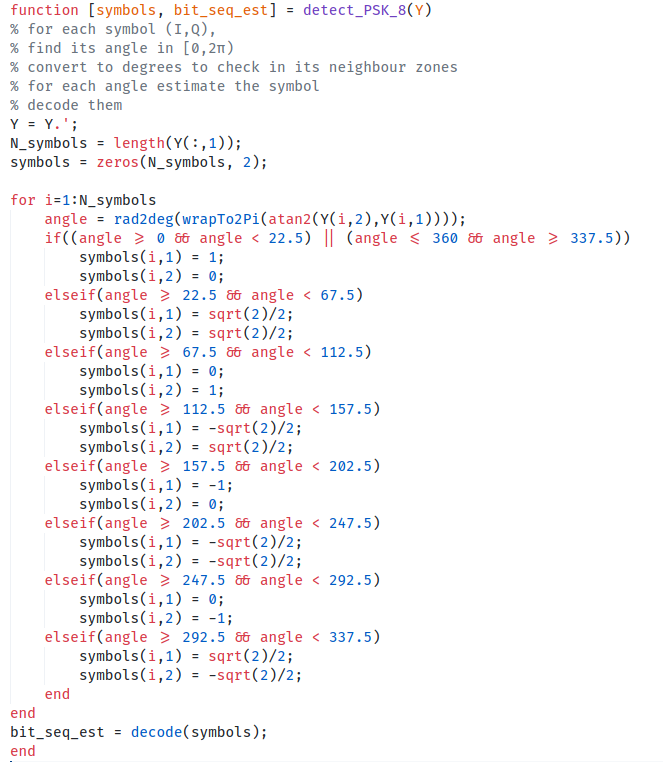
\includegraphics[width=\textwidth]{detect.png}
        \end{figure}
        \begin{figure}[H]
            \centering
            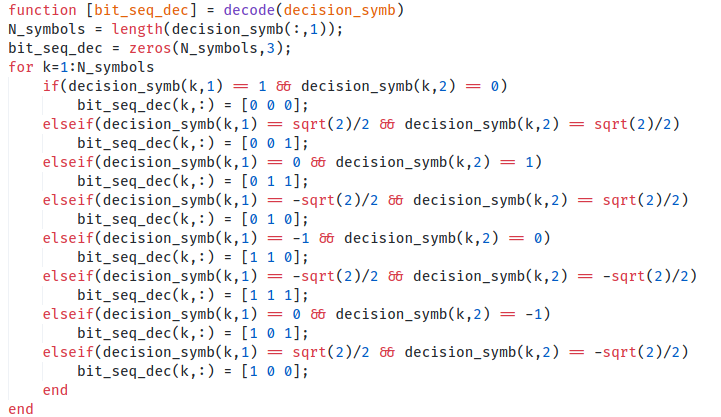
\includegraphics[width=\textwidth]{dec.png}
        \end{figure}
        \item[12.] \underline{Detecting Symbol Errors:}\\
        This function returns how many symbols were falsely Detected. Since MATLAB has different approximations for some functions, rounding was performed
        to avoid false errors being detected
        \begin{figure}[H]
            \centering
            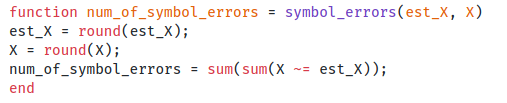
\includegraphics[scale=0.9]{sym_err.png}
        \end{figure}
        \item[13.] \underline{Detecting Bit Errors:}\\
        Just like above, this function detects how many bits were badly decoded.
        \begin{figure}[H]
            \centering
            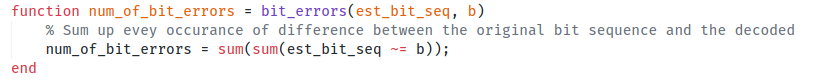
\includegraphics[width=\textwidth]{bit_err.png}
        \end{figure}
    \end{enumerate}
    In the end all the bits and Symbols were received and decoded successfully with zero errors. However an ideal channel was taken for granted and the SNR
    was high.
    \pagebreak
    \item[B.] \textbf{\underline{Probability of Symbol/Bit error estimation using Monte Carlo Method}} 
    \begin{enumerate}
        \item[1.] \underline{Calculate the Error Probabilities for Symbols and Bits alike:}\\
        The code used is the excact same as above with some tweeks to calculate the probability of each SNR value
        (found in monte\_carlo.m script).
        \begin{figure}[H]
            \centering
            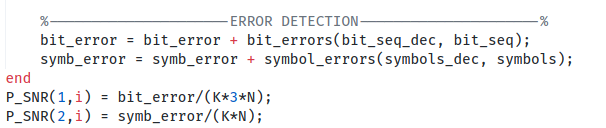
\includegraphics[scale=0.9]{casino.png}
        \end{figure}
        \item[2.] \underline{Symbol's Error Probability Upper Bound: }\\
        The upper bound for \( \textbf{P}(\textbf{E}_{symbol}) \) is given by the following formula:
        \[\textbf{P}(\textbf{E}) \le 2Q\left(\sqrt{2SNR}\sin\left(\frac{\pi}{8}\right)\right),\qquad
        SNR = 10^{\frac{SNR_{dB}}{10}}\]
        \begin{figure}[H]
            \centering
            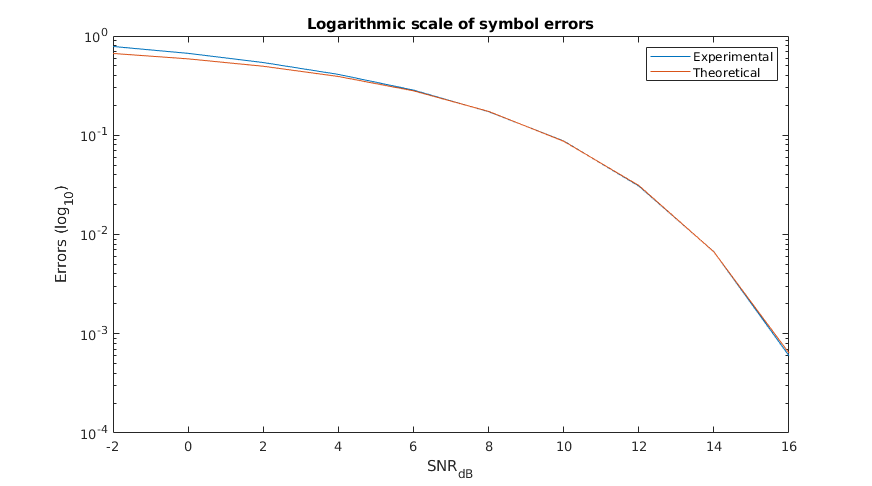
\includegraphics[scale=0.6]{symb_err.png}
        \end{figure}

        \pagebreak
        \item[3.] \underline{Bit's Error Probability Lower Bound: }\\
        The lower bound for \( \textbf{P}(\textbf{E}_{bit}) \) is given by:
        \[\textbf{P}(\textbf{E}_{bit}) \le \frac{2Q\left(\sqrt{2SNR}\sin\left(\frac{\pi}{8}\right)\right)}{3},\qquad
        SNR = 10^{\frac{SNR_{dB}}{10}}\]
        \begin{figure}[H]
            \centering
            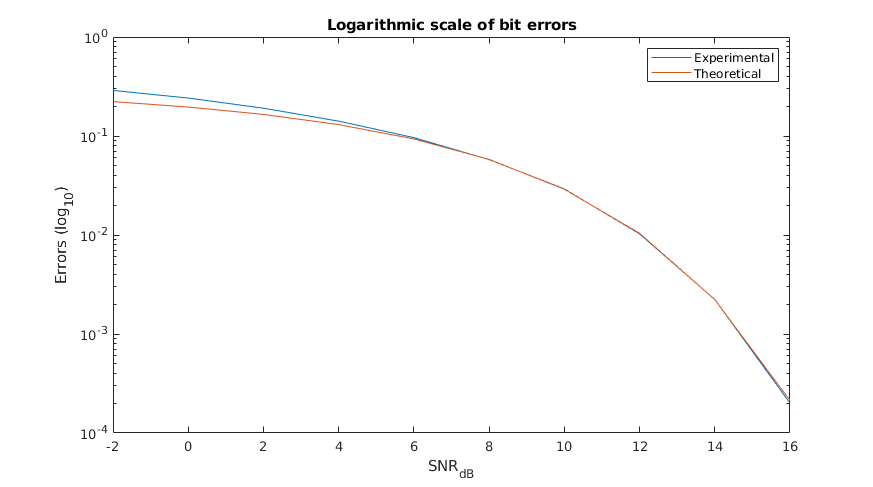
\includegraphics[scale=0.6]{bit_err_.png}
        \end{figure}

        Both experimental bounds match with their theoretical counterparts, although a small divergence can be observed for low values of \(SNR_{db}\)
    \end{enumerate}
\end{enumerate}
\end{document}